\chapter{Evaluation}
\label{chap:eval}

In order to evaluate the quality and effectiveness of the \textcolor{NavyBlue}{\textsc{Solbolt}}, we plan 
to investigate the following categories:

\begin{enumerate}
  \item \textbf{Speed}, in terms of the median and average time needed to analyse a contract
  \item \textbf{Coverage}, in terms of the percentage of EVM bytecode for which the gas estimates can be derived
  \item \textbf{Accuracy}, in terms of the gas estimates calculated
  \item \textbf{User experience}, in terms of the features of the tool and how easy they are to use
\end{enumerate}

To achieve this, we performed a systematic test over a dataset of more than 1000 on-chain Ethereum
smart contracts, collecting key metrics and comparing these with results from previous literature. 
We also performed a case study to illustrate the potential utility of this tool, as explored 
in the next few sections.

\section{Study on coverage and estimation accuracy}

The goal of this study is to provide some insight over points 1, 2 and 3 of our evaluation
criteria --- the speed, coverage and accuracy of our tool. To do this, we ran our extended
Mythril symbolic execution engine
over a dataset containing more than 160,000 verified smart contracts, obtained from 
Etherscan \cite{smart_contract_sanctuary}. However, due to time constraints, we chose to
analyse the top 1,392 smart contracts with the most number of transactions. This also 
allowed the analysed contracts to have a more statistically significant number of concrete
transactions to compare our estimates against, which should allow for lower variance in our
results.

\subsection{Testing pipeline}
First, we obtained the entire index of smart contracts \cite{smart_contract_sanctuary}, 
and sorted it by descending number of transactions. Next, for each smart contract,
we obtained its verified source code using the Etherscan API, and compiled it using
the same compiler settings as the deployed onchain code. We then ran a symbolic execution
instance with the compilation result, using the default settings as shown in Appendix \ref{chap:appendix}.
Each instance is also ran with a symbolic execution timeout of 120 seconds.

Next, after obtaining the symbolic execution results for each contract, we go through and compare the latest 
10,000 transactions, or until 50 valid transactions are obtained, whichever is later. For each concrete
transaction, we extract the function being called from the calldata, as well as the actual gas used
by the transaction. We then, using the estimates from the symbolic execution, calculate the
accuracy of the estimation by dividing it with the concrete gas cost. This means that an accuracy
of 100\% will mean the symbolic execution exactly predicted the concrete gas cost, an accuracy of 125\%
will mean the symbolic execution over-estimated by 25\%, and an accuracy of 75\% will mean the
symbolic execution under-estimated by 25\%. We also calculate the ``gas class" of that transaction,
which sorts the transaction into 9 classes based on its concrete gas cost.
The accuracy for each transaction is then stored, together
with the function it called and its gas class. Afterwards, this routine is repeated for each transaction,
and for each smart contract.
To prevent commonly called functions from skewing the test set, we also limit the maximum number of
analysed transactions for each function to be 30, after which transactions for that function will be ignored.

Finally, the accuracy results are then collated and summarised, by calculating their sum, mean, median
and counts. A summary is also calculated for each function and gas class.
These gas estimation accuracy results, together with the coverage and symbolic execution results, are then stored within a text file,
and will be analysed later. If there are any errors raised
during the entire testing pipeline, it is also logged and stored within the text file.

\subsection{Analysis methodology}

After running the testing pipeline on a sufficient number of smart contracts, we then analysed the 
results using several methods. First, we took the mean gas estimation accuracy and
coverage achieved for each contract, and plotted a violin graph representing the distribution
of data across all smart contracts. We also plotted a histogram of all functions grouped by their
their mean accuracy of predicted gas over concrete gas, and compared this with results from previous literature.

Next, for all smart contracts analysed, we again plotted a violin
graph of mean gas estimation accuracy, but instead grouped them based on the coverage achieved, so
as to observe any correlations between the two. Similarly, this was also done for each transaction,
plotting the mean gas estimation accuracy as a violin graph but grouping them based on their 
``gas class" as mentioned before.

Finally, we plotted a histogram of the number of counts of successful executions, together with 
the counts of various errors encountered, to understand the robustness of the tool under real-world
usage.

\subsection{Results}

The entire evaluation pipeline was run over 51.5 hours on an Intel i7-9700K machine with 32GB DDR4 RAM, 
which was running Ubuntu on Windows Subsystem for Linux, and a total of 1,392 contracts were evaluated.
Of which, 754 contracts were successfully symbolically executed and analysed with their concrete transactions, 
which evalutes to around 4 minutes for each contract. Out of these contracts, 
698 contracts had enough valid concrete transactions for us to
conduct our gas estimation accuracy analysis on, the results of which we shall present in this section.

\subsubsection{Overall coverage and accuracy}

\begin{figure}[h]
  \centering
  \subfloat[\centering Overall gas estimation accuracy (\%)]{{\label{fig:eval_overall_accuracy}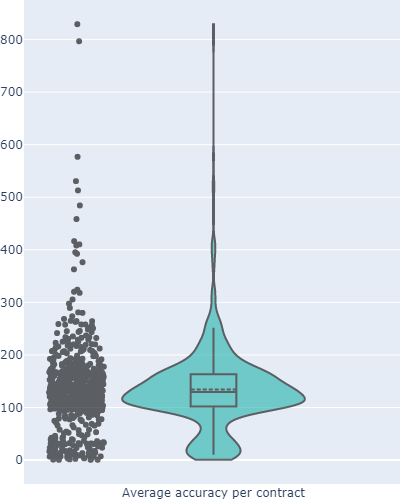
\includegraphics[width=0.4\textwidth]{./figures/eval/overall_accuracy} }}%
  \qquad
  \subfloat[\centering Overall symbolic execution coverage (\%)]{{\label{fig:eval_overall_cov}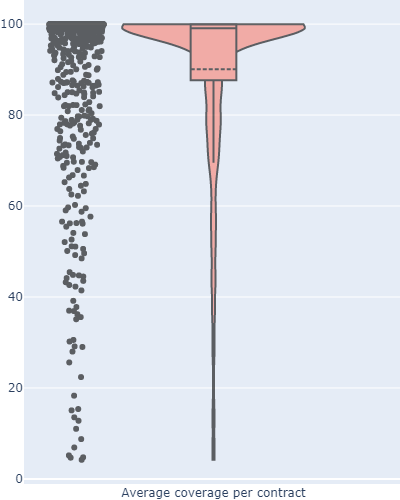
\includegraphics[width=0.4\textwidth]{./figures/eval/overall_cov} }}%
  \caption{Overall results for coverage and accuracy}%
  \label{fig:eval_overall}%
\end{figure}

Overall, across all the analysed smart contracts, the symbolic executor managed to achieve a 
mean gas estimation accuracy of 134.4\%, and a median gas estimation accuracy of 129.3\%.
This is expected, since we are estimating the worst case gas cost of each function, which will
generally be an over-estimate of the concrete gas cost. Examining Figure \ref{fig:eval_overall_accuracy},
we see that the estimation accuracy mostly fall between the 80\% to 200\% range, with the 25th percentile being
102.1\% and the 75th percentile being 163.5\%. We also see very few contracts being severely over-estimated,
although there is a significant density of contracts for which the symbolic executor heavily under-estimates
worst case gas costs. This all suggests that the gas estimation of the symbolic executor is reasonably accurate,
and we believe that the cause for the under-estimation of some contracts is likely due to the lack of coverage.

In addition, the symbolic executor also manages to achieve a mean coverage of 90.1\%, and a median 
coverage of 99.1\%. The 25th percentile achieved for this is 87.6\%, while the 75th percentile is 99.9\%.
This is an impressive result that showcases the performance of our tool, 
since the symbolic executor is still able to cover most code paths
despite facing a limit of 2 symbolic transactions and the execution timeout of 120 seconds.
This is also much better
than the 88\% average and 94\% median coverage achieved by VisualGas, which uses fuzzing and dynamic concrete 
executions instead of symbolic execution as mentioned in Section \ref{section:visualgas}, 
while executing within a similar timeframe. These results also confirm the hypothesis that symbolic execution, which 
analyses a programme path-by-path instead of input-by-input, can be more efficient and achieve greater
coverage for smart contracts, which generally have a large input statespace, but a relatively small executional 
statespace in terms of the range of executed opcodes. 

\subsubsection{Histogram of estimation accuracy per function}

\begin{figure}[h]
  \centering
  \subfloat[\centering Histogram of estimation accuracy for \textcolor{NavyBlue}{\textsc{Solbolt}}]{{\label{fig:eval_fn_accuracy_solbolt}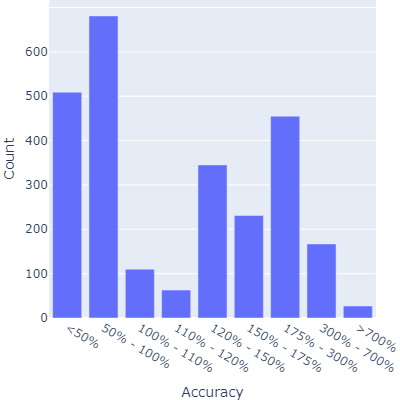
\includegraphics[height=0.2\textheight]{./figures/eval/overall_fn_histogram} }}%
  \qquad
  \subfloat[\centering Histogram of estimation accuracy for \textsc{Gastap}]{{\label{fig:eval_fn_accuracy_GASTAP}\includegraphics[height=0.2\textheight]{./figures/eval/overall_fn_histogram_GASTAP} }}%
  \caption{Estimation accuracy for each function}%
  \label{fig:eval_fn_accuracy}%
\end{figure}

Next, for each function evaluated, we calculated the mean gas estimation accuracy across all transactions,
and binned them into 9 different classes based on their accuracy. These classes are chosen to match those 
evaluated in \textsc{Gastap} \cite{dontrunonfumes}, which we then compared our results against, as shown in
Figure \ref{fig:eval_fn_accuracy}. Unfortunately, as \textsc{Gastap} is closed-sourced and unavailable for 
public testing, we were unable to run the same tests under the same conditions as the ones we 
performed for \textcolor{NavyBlue}{\textsc{Solbolt}}. As such, the published results from the paper were used for comparison instead,
which we were also unable to verify for ourselves.

First, we notice that a far greater number of functions were tested for \textcolor{NavyBlue}{\textsc{Solbolt}} (over 2500 functions) compared to
\textsc{Gastap} (only 125 functions). This may potentially lead to larger possible variability in results for \textsc{Gastap}, especially
if repeated on a similar larger set of contracts.
Next, for a significant proportion of functions, \textcolor{NavyBlue}{\textsc{Solbolt}} still underestimates the 
gas costs required for running them. This can be seen from the bars with estimation accuracy of less
than 100\%, as seen in Figure \ref{fig:eval_fn_accuracy_solbolt}. This is likely because of not having enough coverage
for these functions, possibly due to the max depth being exceeded when executing the path, or hitting the execution timeout.
On the other hand,
\textsc{Gastap} seemed to consistently provide a strict upper bound on gas costs, with zero of the tested functions
recording a concrete gas usage greater than that which was estimated. This is to be expected,
since \textsc{Gastap} makes use of static analysis and reasoning over the generated rule-based representations 
of the bytecode, it is able to produce an over-estimate of the gas cost that is guaranteed to be greater
than the worst case gas usage. In addition, the gas bounds generated by \textsc{Gastap} can be parameterised
by the arguments given, while \textcolor{NavyBlue}{\textsc{Solbolt}} simply executes the contract until the max depth or loop bounds are hit.
This means that for example, if a loop in a smart contract function runs 10 times, the \textsc{Gastap} estimate can take this
into account and calculate an updated worst case gas cost for this. However, if the loop bound limit set for
analysing the same contract in \textcolor{NavyBlue}{\textsc{Solbolt}} was only 5, then \textcolor{NavyBlue}{\textsc{Solbolt}} will likely under-estimate the gas for this function.

For the functions that \textcolor{NavyBlue}{\textsc{Solbolt}} and \textsc{Gastap} over-estimate gas costs for, we see that in \textcolor{NavyBlue}{\textsc{Solbolt}},
the functions are mostly over-estimated by 130\% to 300\%, while in \textsc{Gastap}, the functions
are mostly over-estimated from 100\% to 150\%, when comparing its improved cost models. 
This suggests that \textsc{Gastap} still performs better
at gas estimation than \textcolor{NavyBlue}{\textsc{Solbolt}}, as it is able to provide a stricter and tighter gas upper bound
on a transactional level. However, we believe that \textcolor{NavyBlue}{\textsc{Solbolt}} still performed reasonably well
even when compared to the state-of-the-art of gas bounds estimation. In addition,
\textcolor{NavyBlue}{\textsc{Solbolt}} is capable of tracking gas usage on a per code section basis, rather than simply
on the per-function basis, which provides some additional insight for the developer that \textsc{Gastap}
does not.

\subsubsection{Estimation accuracy by concrete gas usage}

\begin{figure}[h]
  \centering
  \subfloat[\centering Full plot]{{\label{fig:gas_class_acc}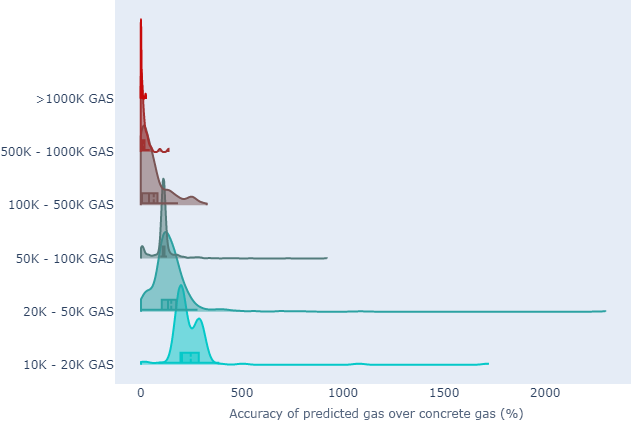
\includegraphics[height=0.22\textheight]{./figures/eval/gas_class_acc} }}%
  \subfloat[\centering Zoomed in]{{\label{fig:gas_class_acc_zoom}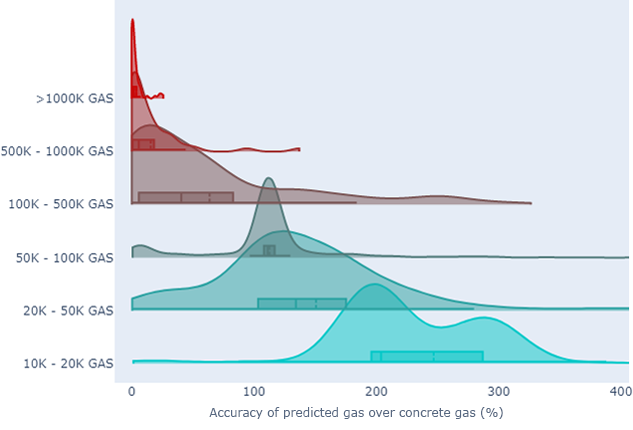
\includegraphics[height=0.22\textheight]{./figures/eval/gas_class_acc_zoom} }}%
  \caption{Estimation accuracy for each gas class}%
  \label{fig:gas_class_accuracy}%
\end{figure}

Next, we also binned each transaction into 6 ``gas classes", based on the concrete amount of 
gas they used in that transaction. We then plotted the estimation accuracy of each transaction, 
grouped by each gas class. This is shown in Figure \ref{fig:gas_class_acc}, with a zoomed in view
shown in Figure \ref{fig:gas_class_acc_zoom}. Here, we observe a trend where the higher the
concrete gas cost is, the lower the percentage of the estimated gas cost over the concrete cost is.
This may be directly because of the max depth and loop bounds limit imposed on the execution.
For transactions that have very high gas usage, it is likely that they may be running many iterations
of a loop, far greater than the loop bounds set in the symbolic execution. As such, the gas
estimate generated by \textcolor{NavyBlue}{\textsc{Solbolt}} will also likely be an underestimate. For transactions with very
little gas usage, the inverse may be true. They may be taking paths through the function that require
less gas, or possibly run very few iterations through a loop. This makes it likely for \textcolor{NavyBlue}{\textsc{Solbolt}}
to over-estimate the gas used. 

We can clearly see that precisely estimating the concrete gas used
by every transaction is not a trivial task, as each this depends on the exact state of the contract, 
as well as the parameters given. However, the results also show that the
median gas estimation accuracy for gas classes ranging from 10,000 gas units to 500,000 gas units,
which cover the vast majority (94.4\%) of all transactions tested,
are still relatively reasonable, ranging from an mean of 40.6\% to 204.1\% of the concrete gas costs. 
We believe that this makes the gas estimation from \textcolor{NavyBlue}{\textsc{Solbolt}} still insightful for developers.
Developers can also tweak the limits of the symbolic executor to match what is expected
from their functions, which can potentially produce more accurate estimates.

\subsubsection{Estimation accuracy by coverage}

\begin{figure}[h]
  \centering
  \subfloat[\centering Full plot]{{\label{fig:cov_class_acc}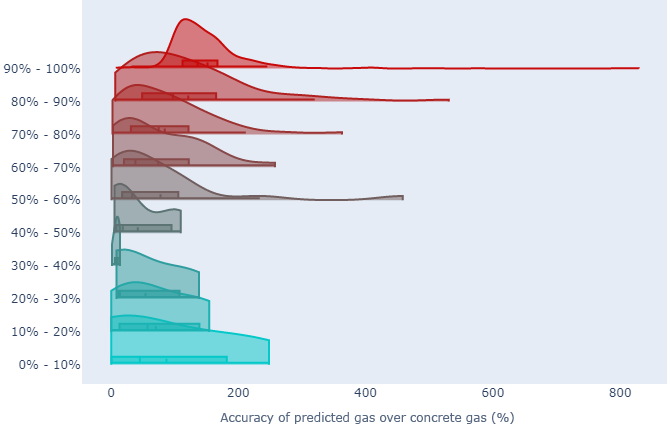
\includegraphics[height=0.207\textheight]{./figures/eval/cov_acc} }}%
  \subfloat[\centering Zoomed in]{{\label{fig:cov_class_acc_zoom}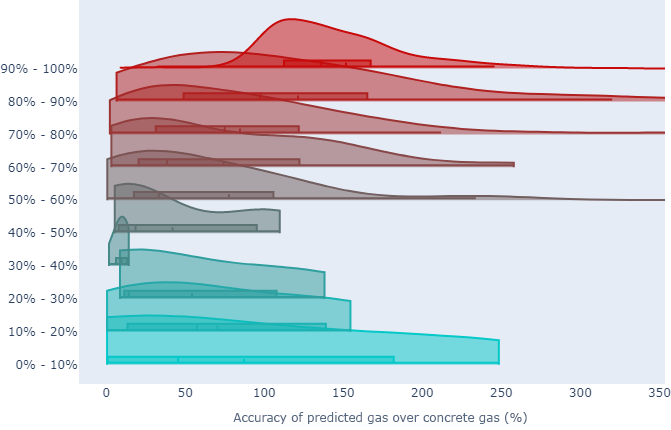
\includegraphics[height=0.207\textheight]{./figures/eval/cov_acc_zoom} }}%
  \caption{Estimation accuracy for each coverage class}%
  \label{fig:cov_class_accuracy}%
\end{figure}

We again plotted a similar graph of estimation accuracy, this time grouped via 10 coverage classes instead,
sorted based on the overall coverage achieved for each contract. The estimation accuracy is also
taken from the mean estimation accuracy of all transactions for each contract, rather than the
per transaction accuracy as before. The graph is shown in Figure \ref{fig:cov_class_acc},
with a zoomed in view shown in Figure \ref{fig:cov_class_acc_zoom}. 

Here, we observe the trend that where the lower the coverage is, 
the lower the percentage of the estimated gas cost over the concrete cost is.
This is to be expected, given that the gas estimation depends entirely on
how much of the contract is executed. This also adds support to our theory that
the lack of coverage is the main reason why \textcolor{NavyBlue}{\textsc{Solbolt}} underestimates gas costs for
certain contracts. This lack of coverage could occur for several reasons, such as
if the max depth or call limit is hit when executing a certain path. If the Z3 solver
was enabled, this could also happen because the solver timeout was reached, or if
the solver determines a certain code path was unreachable.

We also see that for the class
containing 90\% to 100\% coverage (which covers 73.7\% of all contracts),
the median gas estimation accuracy is 136.2\%. This implies that \textcolor{NavyBlue}{\textsc{Solbolt}} does tend to produce an
over-estimate of the gas cost, if the contract is well-covered. For the classes containing
80\% to 90\% and 70\% to 80\% coverage (covering a total of 14.9\% of all contracts),
the median gas estimation accuracy drops to 97.5\% and 74.9\% respectively. This is likely because
although \textcolor{NavyBlue}{\textsc{Solbolt}} generally over-estimates the gas cost, the lower coverage offsets this effect,
resulting in a slight under-estimate of gas costs instead. Similarly, this test was run with
the same symbolic execution settings for all contracts, and users are encouraged to tweak the
settings to the requirements of their own contracts.

\subsubsection{Histogram of success and error rates}

\begin{figure}[h]
  \centering
  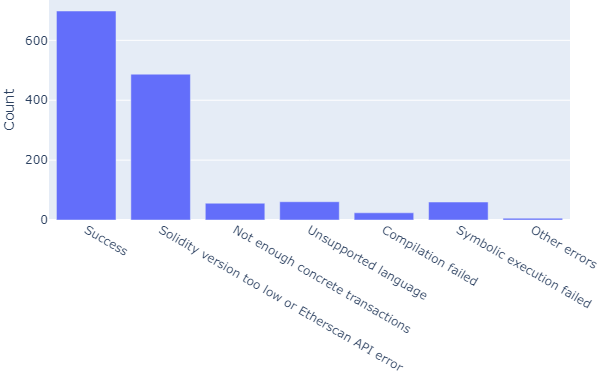
\includegraphics[width=0.8\textwidth]{./figures/eval/eval_status}
  \caption{Evaluation status}
  \label{fig:eval_status}
\end{figure}

Finally, we plotted a graph of the final evaluation status --- whether it was
successful, or which error was caught while evaluating --- for each of the 1,392
contracts tested, as shown in Figure \ref{fig:eval_status}. As shown in the graph,
698 contracts were successfully evaluated, while 694 contracts caught an error 
during the evaluation pipeline. Out of this, the vast majority of errors (487) were because
the Solidity compiler versions of the smart contracts were lower than version 0.4.17. These compilers were not
supported, because they still lacked the functionality to 
produce an abstract syntax tree, which was required for the symbolic execution. In addition, 
56 contracts were discarded for having not enough concrete transactions (and hence datapoints) 
for evaluation, 61 contracts were discarded for not being written in Solidity, and 6 contracts
were caught with other errors. 

This left a remaining 24 contracts faced with compilation errors,
and 60 contracts faced with a symbolic execution error. For the compilation errors,
these were mainly due to some contracts manually linking certain libraries, which is
not yet supported by \textcolor{NavyBlue}{\textsc{Solbolt}}, or because of import errors. For the symbolic execution errors,
these occured primarily due to the contract creation transaction not being able to
deploy the contract and construct the initial open states. This could in turn be because
the max depth was hit during the constructor of the contract, or the executor timing out.

Only counting the errors faced with symbolic execution and compilation, we have an overall
evaluation success rate of 89.3\%. While this certainly could be improved upon, we believe
that the tool is still very reliable for general usage. In addition, many of the errors
are from testing on older smart contracts, whereas the tool was designed with the newer features
of more recent compiler versions in mind. As such, while the tool still mostly supports 
the wide range of compiler versions we have available, contracts written with more recent 
versions of Solidity are much less likely to face problems while using the tool.

\section{Case Study: Gas-hungry loops}
\label{section:gas_hungry_loop}

Next, we present a case study on three contracts, to investigate how 
a user might make use of \textcolor{NavyBlue}{\textsc{Solbolt}} to optimise their code. The goal of this
study is to provide some insight to the utility of this tool, and how a
developer might use the available information to optimise a smart contract.

\subsection{A really gas-hungry loop}

\begin{lstlisting}[language=Solidity, caption={A really gas-hungry loop contract}, label={lst:eval_contract_1}, basicstyle=\ttfamily\scriptsize]
  // SPDX-License-Identifier: GPL-3.0
  pragma solidity >=0.7.0 <0.9.0;
  contract GasHungryLoop {
      mapping (uint256 => address) private tokenToOwner;
      uint256 indexToMint;

      function mint(uint256 numberToMint) external {
        for (uint256 i = 0; i < numberToMint; i++) {
          tokenToOwner[indexToMint++] = msg.sender;
        }
      }
  }
\end{lstlisting}

Let us examine the above smart contract, as shown in Listing \ref{lst:eval_contract_1}. 
This contract is a stripped down version of a standard ERC-721 non-fungible token (NFT) contract,
where only a mapping from the token ID to the owner address is stored. The other functions typically
required for an ERC-721 token, such as \texttt{transferFrom}, \texttt{approve} and \texttt{tokenURI}, 
are not included here for brevity. Here, the mint function will ``mint" a certain
number of NFTs, by iterating through the loop \texttt{numberToMint} times, and each time
setting the owner of the token ID to the sender of the transaction. After each iteration, \texttt{indexToMint}
will be incremented and stored, so the contract knows what is the next token ID it should assign.

This contract is written in a highly concise way, similar to how a non-blockchain programme
might be written. However, after running the symbolic execution (with settings listed in Appendix \ref{chap:appendix}), we notice a few problems,
as shown in Figure \ref{fig:eval_case_issues}.

\begin{figure}[h]
  \centering
  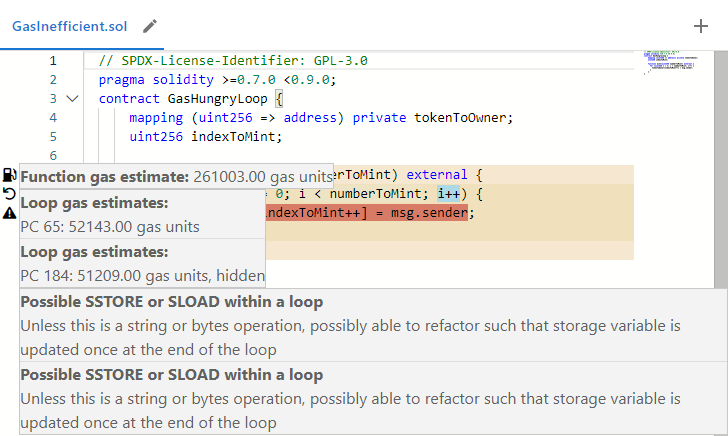
\includegraphics[width=0.8\textwidth]{./figures/eval/case_issues}
  \caption{Gas estimates and issues detected by \textcolor{NavyBlue}{\textsc{Solbolt}}}
  \label{fig:eval_case_issues}
\end{figure}

Here, we see that the gas estimate for the
\texttt{mint} function (assuming a loop bounds of 5) is 261,003 gas units, which is
relatively high for a single transaction. We also see that the symbolic execution engine
detected two loops from lines 8 to 10. The first loop, with a per-iteration gas cost of
52,143 gas units, is likely to be the \texttt{for} loop written within these lines.
This is in line with the overall function gas estimate when multiplied by the loop bounds
(five times of the per-iteration gas cost would be 260,715, slightly below the estimated function gas cost), 
as most of the gas would be consumed by the loop (which makes up majority of the function).
The second loop, with a per-iteration gas cost of 51,209 gas units, is a hidden loop
that is executed within the for loop, and is likely generated by the compiler because
of the access of a mapping structure here.



We also see that there are two warnings for a possible SSTORE or SLOAD within a loop,
on line 9. This suggests that it may be possible to refactor the code such that
storage variables are not accessed on each iteration, but rather updated once
at the end of the loop by making use of temporary local variables.
This is precisely the case here, since we both read from and increment the 
\texttt{indexToMint} variable, which is a storage variable, at each loop iteration.

\begin{figure}[h]
  \centering
  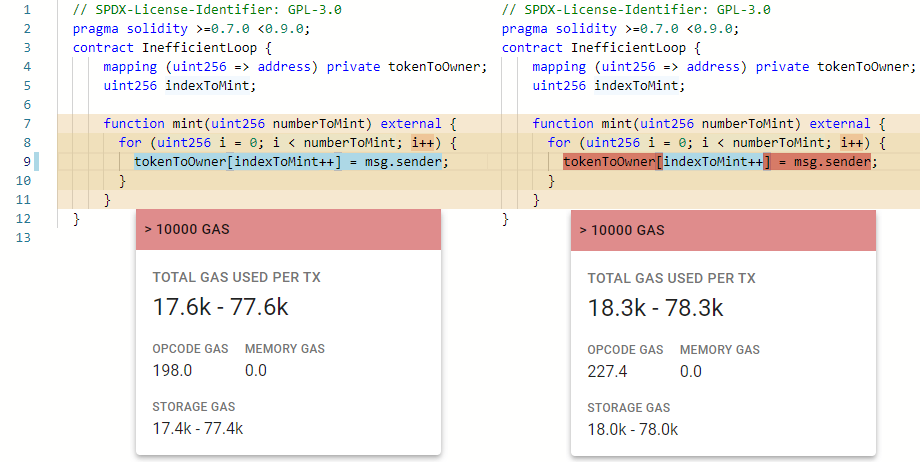
\includegraphics[width=0.8\textwidth]{./figures/eval/case_gas}
  \caption{Two code sections with very high estimated gas costs}
  \label{fig:eval_case_gas}
\end{figure}

Hovering over them to see their precise gas estimates for each code section as seen 
in Figure \ref{fig:eval_case_gas}, we also
see that the two storage updates to the \texttt{tokenToOwner} mapping and 
\texttt{indexToMint} integer can take over 77k gas units, which makes up the majority
of all gas consumed in the loop. This suggests to the developer that optimising these
storage updates could provide a significant gas saving.

Indeed, one idea could be to make use of the \texttt{i} local variable during each loop iteration
for indexing the mapping, and then increment the \texttt{indexToMint} variable with \texttt{i} 
at the end. Since each transaction on the EVM is executed sequentially, there is no concern
for race conditions with other contract interactions sent at the same time.


\subsection{A more optimised loop}

\begin{lstlisting}[language=Solidity, caption={A more optimised loop contract}, label={lst:eval_contract_2}, basicstyle=\ttfamily\scriptsize]
  // SPDX-License-Identifier: GPL-3.0
  pragma solidity >=0.7.0 <0.9.0;
  contract SlightlyBetterLoop {
      mapping (uint256 => address) private tokenToOwner;
      uint256 indexToMint;

      function mint(uint256 numberToMint) external {
        for (uint256 i = 0; i < numberToMint; i++) {
          tokenToOwner[indexToMint + i] = msg.sender;
        }
        indexToMint += numberToMint;
      }
  }
\end{lstlisting}

Using the approach outlined before, we have this newer, more optimised contract,
as shown in Listing \ref{lst:eval_contract_2}. Running the symbolic execution again gives
the following result, as shown in Figure \ref{fig:eval_case_issues_better}.

\begin{figure}[h]
  \centering
  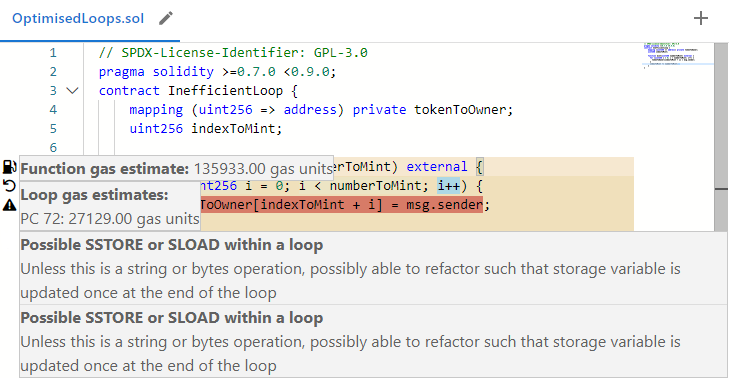
\includegraphics[width=0.8\textwidth]{./figures/eval/case_issues_better}
  \caption{Gas estimates and issues for more optimised loop}
  \label{fig:eval_case_issues_better}
\end{figure}

Here, we see that now, the function gas estimate has dropped to just 135,933 gas units,
which is a improvement of 47.9\% over the non-optimised contract. The per-iteration gas
cost has also improved by a similar amount to just 27,129 gas units. Examining the
gas estimates of the same two costly sections identified previously, as displayed
in Figure \ref{fig:eval_case_gas_better}, we see that the gas cost for
calculating the index of the mapping has reduced greatly to just 266 gas units.
The gas estimate for updating the mapping itself has not changed, as it cannot be
refactored, due to it being a necessary operation of this function.

\begin{figure}[h]
  \centering
  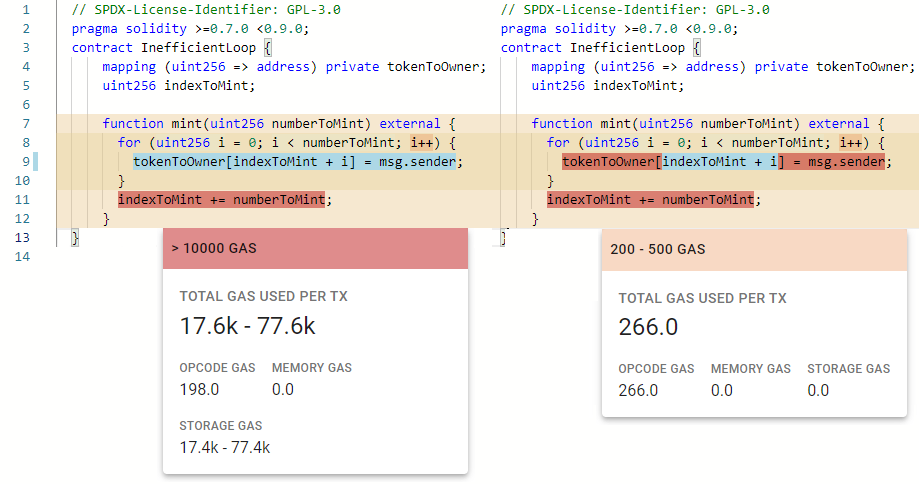
\includegraphics[width=0.8\textwidth]{./figures/eval/case_gas_better}
  \caption{Optimised costs for the two gas-hungry code sections identified}
  \label{fig:eval_case_gas_better}
\end{figure}

However, we still see that there are two warnings for the use of \texttt{SSTORE} or \texttt{SLOAD} 
within the loop. This suggests that there may still be further gas savings achievable. Indeed,
we are still reading the \texttt{indexToMint} storage variable within the loop, albeit
no longer updating it. 

The most optimised solution to this would therefore be to store a temporary copy
of the \texttt{indexToMint} variable, and then simply working with this within the loop, before 
finally updating the actual storage variable at the end of the loop, as seen in Listing 
\ref{lst:eval_contract_3}. However, this gas saving comes at a cost of verbosity and
readability, which the developer needs to carefully balance while creating a contract.

\begin{lstlisting}[language=Solidity, caption={The most optimised loop contract}, label={lst:eval_contract_3}, basicstyle=\ttfamily\scriptsize]
  // SPDX-License-Identifier: GPL-3.0
  pragma solidity >=0.7.0 <0.9.0;
  contract InefficientLoop {
      mapping (uint256 => address) private tokenToOwner;
      uint256 indexToMint;

      function mint(uint256 numberToMint) external {
        uint256 i = indexToMint;
        uint256 limit = i + numberToMint;
        for (; i < limit; i++) {
          tokenToOwner[i] = msg.sender;
        }
        indexToMint += numberToMint;
      }
  }
\end{lstlisting}

\subsection{Other examples}

Through this case study, we have successfully demonstrated how in this particular case,
a developer can make use of the gas insights provided to optimise a gas-inefficient
loop pattern. In addition, we also provide 3 other examples for users to explore,
illustrating issues such as the ordering of storage variables, the use of recursion,
and the effect of public functions on the dispatcher routine. These are all available
within the ``Examples" tab on the live website. 

We believe that these are a useful
starting point for developers learning to use \textcolor{NavyBlue}{\textsc{Solbolt}},
allowing them to better make use of the detailed gas cost breakdown and potential
issues provided by \textcolor{NavyBlue}{\textsc{Solbolt}} to identify problems in their own smart contracts.